\chapter{Analyse}

\section{Akt�rer}

Der er f�lgende akt�rer i systemet:

\textbf{Administrator}: Han har mulighed for at se alle beskeder i g�stebogen, ogs� selvom de er skjulte. Derudover har han mulighed for at administrere g�stebogens forskellige beskeder, ved at slette eller skjulte dem der ikke er relevante for ham og/eller brugerne.

\textbf{G�stebogs brugere}: Brugeren har mulighed for at skrive en lille anmeldelse af deres ophold p� g�rden, ved at indtaste navn, vurdering og en besked, der vil blive gemt og vist i g�stebogen for andre brugere, medmindre administratoren v�lger at skjule/slette disse.

\section{Use cases \& scenarier}
 
\begin{itemize}
\item \emph{Brugeren} skriver en besked. (Han tilf�jer sit navn, en vurdering og en besked)
\item \emph{Administratoren} sletter en besked fra g�stebogen.
\item \emph{Administratoren} skjuler en besked I g�stebogen.
\item \emph{Administratoren} v�lger hvilken g�stebog der er aktuelt vist for brugeren.
\end{itemize}

\subsection{Scenarie for bruger}

Brugeren vil gerne skrive en anmeldelse af sit ophold. De �bner g�stebogs-applikationen, hvor de har mulighed for at indtaste deres navn, vurdering af opholdet, samt et besked.

Herefter kan de sende beskeden som bliver oprettet og vist i en ny fane under \emph{Se beskeder}. Her har de mulighed for at se deres besked, sammen med beskeder fra andre brugeres tidlige ophold.

\subsection{Scenarie for administrator}

Administratoren v�lger at g� ind i administrator-panelet, hvor han har nogle forskellige muligheder. Han kan se beskederne i den aktuelt valgte g�stebog, han kan v�lge beskeder ud som han vil skjule eller slette og han har derudover mulighed for at �ndre hvilken g�stebog der er aktuelt vist for brugeren.

\section{Objektmodel}

Figur \ref{object-model} viser eksempler p� objekter i systemet.

\begin{figure}[h]
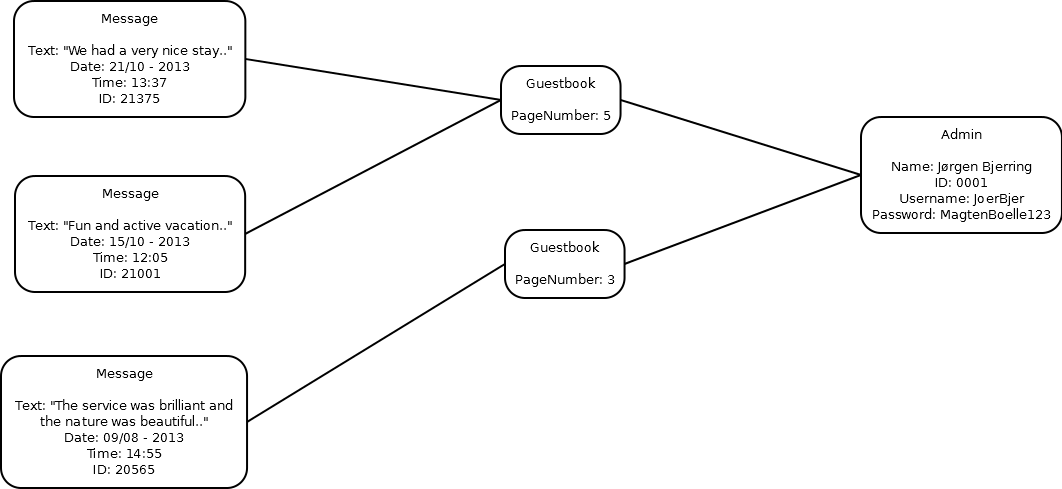
\includegraphics[width=\linewidth]{./object-model}
\caption{Objektmodel for den digitale g�stebog}
\label{object-model}
\end{figure}

\section{Dom�nemodel}

Figur \ref{domain-model} viser dom�nemodellen for systemet.

\begin{figure}[h]
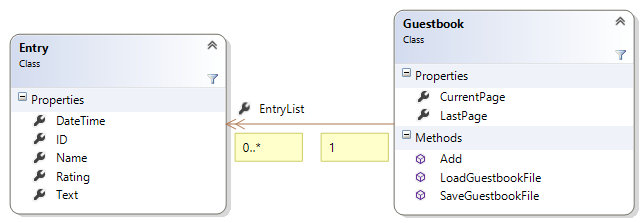
\includegraphics[width=\linewidth]{./domain-model}
\caption{Dom�nemodel for den digitale g�stebog}
\label{domain-model}
\end{figure}
